\documentclass[]{IEEEtran}

\usepackage[english,portuguese]{babel}
\renewcommand{\IEEEkeywordsname}{Palavras-chave}

\usepackage{float}
\usepackage{graphicx,url}
\usepackage{caption}
\usepackage[T1]{fontenc}
\usepackage{tgbonum}
%%\usepackage{setspace}

\ifCLASSINFOpdf

\else

\fi

\hyphenation{op-tical net-works semi-conduc-tor}


\begin{document}

\title{Análise do teorema\\ PAM natural}

\author{Antônio~Raian,~UEFS,
        Gustavo~Henrique,~UEFS,
        and~Lucas C. A. Lima,~UEFS% <-this % stops a space
\thanks{M. Shell was with the Department
of Electrical and Computer Engineering, Georgia Institute of Technology, Atlanta,
GA, 30332 USA e-mail: (see http://www.michaelshell.org/contact.html).}% <-this % stops a space
\thanks{J. Doe and J. Doe are with Anonymous University.}% <-this % stops a space
\thanks{Manuscript received April 19, 2005; revised August 26, 2015.}}


\markboth{Journal of \LaTeX\ Class Files,~Vol.~14, No.~8, August~2015}%
{Shell \MakeLowercase{\textit{et al.}}: Bare Demo of IEEEtran.cls for IEEE Journals}

\maketitle

\begin{abstract}
Este artigo apresenta os procedimentos envolvidos na análise de um sinal analógico com o objetivo de realizar operações que facilitem sua reconstrução precisa. Os passos incluem a aplicação de um filtro de entrada para extrair informações em uma faixa de frequência específica, a conversão do sinal para o domínio do tempo discreto (C/D), a aplicação de um filtro de saída para otimizar o processo de reconstrução e, finalmente, a posterior reconversão para o domínio do tempo contínuo (D/C). Esses procedimentos são cruciais para assegurar a fidelidade na reconstrução do sinal analógico.
\end{abstract}

\begin{IEEEkeywords}
Amostragem de Sinais, Conversão de Sinais, Filtragem de Sinais.
\end{IEEEkeywords}


\IEEEpeerreviewmaketitle



\section{Introdução}

\IEEEPARstart{N}{o} âmbito da aquisição e processamento de sinais, o trabalho de amostragem e recuperação de um sinal analógico contínuo no tempo desempenha um papel fundamental. A forma mais comum de encontrar informações na natureza é através de sinais analógicos (contínuos no tempo) tais como, ondas sonoras, luz, temperatura, corrente elétrica e etc. No entanto, quando se trata de manipular e analisar estas informações utilizando ferramentas computacionais, há uma limitação destas máquinas em lidar diretamente com este tipo de sinais. É neste contexto que o teorema da amostragem se torna essencial. 

Este teorema possibilita a discretização de um sinal analógico, transformando-o em uma representação matemática que pode ser facilmente processada e analisada. Neste artigo, exploraremos os procedimentos envolvidos na aplicação do teorema da amostragem para converter e reconstruir sinais analógicos, destacando sua importância no contexto da engenharia de sinais e processamento de dados.

\section{Fundamentação teórica}

\subsection{Teorema da amostragem}

O sinal de forma discreta no tempo pode ser obtido de formas distintas, uma delas é a partir da amostragem de sinais contínuos$^{[1]}$. Um sinal contínuo no tempo deve estar em sua forma discretizada para que possa ser analisado por uma máquina, pois esta não consegue analisar o sinal em todo o domínio do tempo. Desta forma, o sinal deve ser lido através pontos específicos.

\subsubsection{PAM (Modulação por Amplitude de Pulso)}
Uma das técnicas utilizadas para realizar a amostragem é através do PAM (\textit{Pulse Amplitude Modulation}). O PAM é uma técnica de modulação usada para transmitir sinais analógicos ou digitais em sistemas de comunicação digital. Envolve amostrar o sinal em intervalos regulares, multiplicando o sinal por um trem de pulsos retangulares (amostragem natural) ou de impulsos unitários (amostragem ideal).

A equação (\ref{eq:produtotremdeimpulsos}) representa a expressão matemática descrita pelo produto entre o sinal e um trem de impulsos, tendo como resultado o sinal amostrado $x_{s}(t)$ formado por impulsos de mesma amplitude das amostras do sinal $x(t)$.

\begin{equation}\label{eq:produtotremdeimpulsos}
    x_{s}(t) = x(t) \cdot p(t)
\end{equation}

\begin{equation}\label{eq:tremdeimpulsos}
    p(t) = \sum_{n=-\infty}^{\infty} \delta(t - nT)
\end{equation}

\subsection{Efeito da subamostragem: Aliasing}

\subsubsection{Aliasing}

A escolha da frequência de amostragem é um ponto importante ao amostrar um sinal contínuo, pois pode acabar comprometendo a sua reconstrução. Caso a frequência de amostragem não seja suficientemente alta, ocorre uma sobreposição de espectros durante o fenômeno de replicação da faixa de frequência original do sinal.

\subsubsection{Filtro passa-baixas}

Na maioria das vezes quando um sinal de frequência é recebido para o processamento e análise, a sua informação está contida em uma faixa de frequência com extensão finita, sendo assim, há a necessidade de um sistema que possa fazer a seleção da frequência, limitando o seu espectro à faixa que desejada. Este processo é feito através de filtros.

Os filtros são caracterizados por limitar uma faixa de passagem do sinal rejeitando outra parte. Haykin e Veen em sua obra definem que:

\begin{quote}
    "Sinais com frequências dentro da faixa de passagem, são transmitidos com pouca ou nenhuma distorção, ao passo que aqueles que têm frequências dentro da faixa de rejeição são efetivamente rejeitados".
\end{quote}

O filtro passa-baixas ideal permite a transmissão de baixas frequências atenuando a amplitude que sejam maior que a sua frequência limite, conhecida como frequência de corte. Considerando o ambiente como ideal, o ganho do filtro é unitário, ou seja o módulo do sinal de entrada é igual a sua saída, e para frequência acima de sua frequência de corte, o sinal é atenuado a zero. Porém, este tipo de resposta não é obtido na prática.

\subsubsection{Teorema de Nyquist-Shannon}

Pelo teorema de Nyquist, para que um sinal contínuo limitado em banda seja completamente reconstruído a partir de uma sequência finita de amostras, é necessária que sua taxa de amostragem seja pelo menos duas vezes maior que a frequência máxima do sinal tal como mostra a equação (\ref{eq:nyquist}):

\begin{equation}\label{eq:nyquist}
    \omega_{m} > 2 \cdot \omega_{s}
\end{equation}

Esse critério é dado pois as rélicas do sinal podem causar a sobreposição dos espectros como citado anteriormente, provocando o efeito de \textit{aliasing}, impedindo assim a reconstrução do sinal inicial. Uma forma de evitar este efeito, caso a frequência de amostragem não obedeça o teorema de Nyquist, é a partir da implementação de um filtro passa-baixas localizado antes da discretização do sinal, limitando a máxima frequência à metade da frequência de amostragem. Este filtro é chamado de filtro \textit{anti-aliasing}.

\subsection{Transformada de Fourier}
Uma das maneiras de analisar os sinais no espectro da frequência é utilizando a transformada de Fourier. Essa ferramenta permite que possamos, matematicamente, decompor o sinal do tempo e observar as suas componentes na frequência. A Transformada de Fourier de um sinal $x(t)$ é dada por:

\begin{equation}
     X(f) = \int_{-\infty}^{\infty} x(t) e^{-j2\pi ft} dt
\end{equation}
onde \(X(f)\) é o espectro de frequência do sinal e \(f\) é a frequência.

Uma vez que já possuímos o sinal discretizado, decompô-lo na frequência pode ficar mais viável utilizando-se da \textit{Transformada Rápida de Fourier} (FFT). Essa, por sua vez, é dada por:
\begin{equation}
    X(k) = \sum_{n=0}^{N-1} x(n) e^{-j2\pi kn/N} 
\end{equation}
onde \(X(k)\) representa o espectro de frequência discreto, \(x(n)\) são as amostras do sinal e \(N\) é o número de amostras.

Ainda no âmbito discreto, é possível, a partir das componentes de frequência, reconstruir o sinal no tempo. Para tal é preciso fazer o caminho inverso da transformada de Fourier. Este é o papel da \textit{Transformada Rápida Inversa de Fourier} (IFFT). A IFFT é definida como:
\begin{equation}
    x(n) = \frac{1}{N} \sum_{k=0}^{N-1} X(k) e^{j2\pi kn/N}
\end{equation}
onde \(x(n)\) representa as amostras do sinal no domínio do tempo e \(X(k)\) é o espectro de frequência discreto.

\section{Metodologia}

Este projeto foi realizado através da linguagem de sintaxe matemática Octave. Esta linguagem disponibiliza diversas ferramentas e bibliotecas direcionadas ao processamento de sinais, permitindo a aplicação de transformadas rápidas, filtragem e construção de gráficos. A partir disto, foi possível definir o diagrama geral do projeto:

\begin{figure}[H]
\captionsetup{justification=centering}
\centering % para centralizarmos a figura
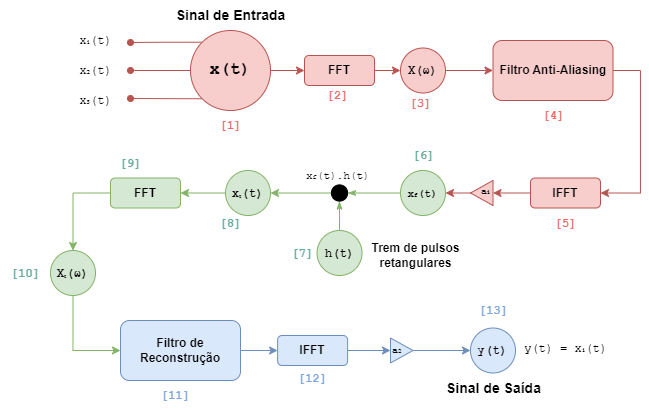
\includegraphics[width=9cm]{Diagrama_Geral.png} % leia abaixo
\caption{Diagrama geral do projeto com seus componentes enumerados e setores divididos em cores}
\end{figure}

Como é ilustrado pela figura acima, o diagrama é dividido em três setores caracterizados por suas respectivas cores. Em vermelho, encontra-se a etapa de filtragem do sinal de entrada. Em seguida, em verde, a etapa de amostragem. Por fim, em azul, a etapa de reconstrução de sinal. Esta diferenciação foi aplicada meramente para fins didáticos. 

\subsection{Filtragem do Sinal de Entrada}

\subsubsection{Sinal de Entrada}

O sinal de entrada$^{[1]}$ é formado a partir da soma de diferentes senóides com suas respectivas frequências. Tomando como exemplo o diagrama do projeto, a primeira senóide ($x_1$) é o sinal que se deseja filtrar, enquanto que as demais ($x_2$ e $x_3$) representam, neste caso, ruídos indesejáveis. 

\subsubsection{Sinal de Entrada na frequência}

Antes de filtrar o sinal de entrada, é necessário convertê-lo para o domínio da frequência. Para isto, pode-se utilizar a transformada rápida de fourier$^{[2]}$, representada pelo comando {\fontfamily{pcr}\selectfont fft} no Octave. Através dela, obtém-se o espectro de frequência do sinal, que é formado a partir de cada frequência das $n$ senóides que compõem $x(t)$.

\begin{figure}[H]
\captionsetup{justification=centering}
\centering % para centralizarmos a figura
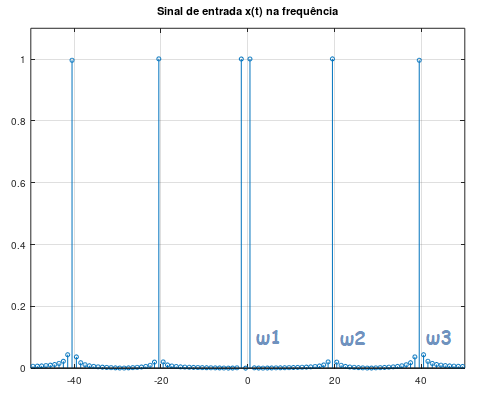
\includegraphics[width=4cm]{ex_sinal_entrada_freq.png} % leia abaixo
\caption{Componentes de frequência do sinal $x(t)$.}
\end{figure}

\subsubsection{Filtrando o Sinal de Entrada}

A fim de remover possíveis frequências indesejáveis, utiliza-se um filtro \textit{anti-aliasing} ideal$^{[4]}$. Matematicamente, este filtro nada mais é que uma função retangular de pulso único, representado no Octave pelo comando {\fontfamily{pcr}\selectfont rectpuls}. 

Efetuar um produto entre $X(\omega)$ e o filtro $rect(\omega)$ significa eliminar todas as frequências que não se encontram no intervalo definido pela área retangular. 

\begin{figure}[H]
\captionsetup{justification=centering}
\centering % para centralizarmos a figura
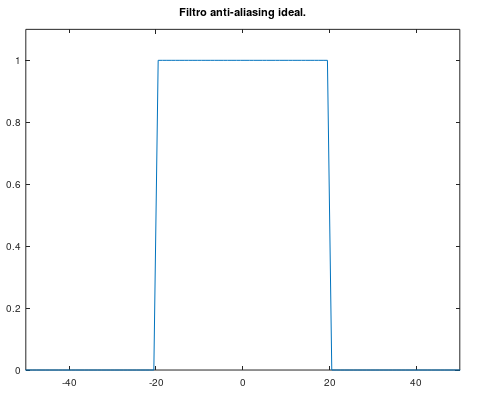
\includegraphics[width=3cm]{ex_filtro_aliasing.png} % leia abaixo
\caption{Exemplo de um filtro ideal $rect(\omega)$.}
\end{figure}

Quanto maior for a largura do pulso, mais informação do sinal original ele filtrará. Em outras palavras, se a largura do filtro tender ao infinito, todo o espectro de frequência será recuperado.

\begin{figure}[H]
\captionsetup{justification=centering}
\centering % para centralizarmos a figura
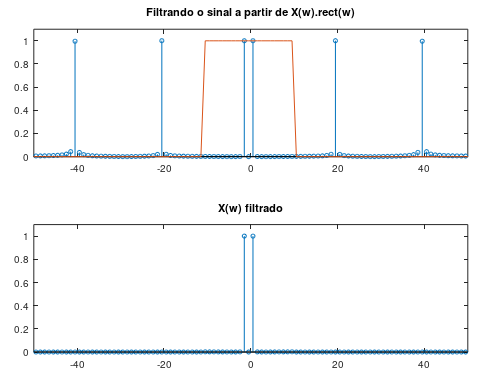
\includegraphics[width=4cm]{ex_filtrando.png} % leia abaixo
\caption{Representação gráfica do processo de filtragem. Nesta situação, a frequência $\omega$$_1$ foi filtrada.}
\end{figure}

\subsubsection{Retornando para o domínio do tempo}

Após filtrar o sinal, basta retornar para o domínio do tempo. Para isto, utiliza-se a transformada rápida inversa de fourier$^{[5]}$, cujo comando no Octave é {\fontfamily{pcr}\selectfont ifft}. Uma vez que o sinal de entrada filtrado $x$$_f$$(t)$ é reconstruído, o resultado gráfico no tempo deve ser semelhante a curva senoidal correspondente à frequência filtrada. Além disso, o processo de filtragem e reconstrução gera atenuação na amplitude do sinal, portanto é necessário fazer uma amplificação no sinal $x$$_f$$(t)$ para uma melhor aproximação a senóide desejada.

\begin{figure}[H]
\captionsetup{justification=centering}
\centering % para centralizarmos a figura
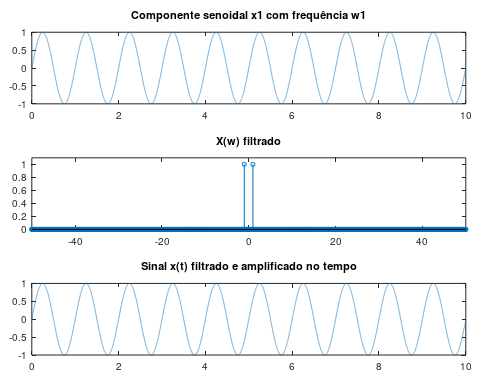
\includegraphics[width=4cm]{ex_amplificando.png} % leia abaixo
\caption{Comparação gráfica entre o componente senoidal $x_1$ e o sinal $x$$_f$$(t)$.}
\end{figure}

\subsection{Amostragem do Sinal}

\subsubsection{Trem de pulsos retangulares}

Seguindo a ordem estabelecida pelo diagrama, tem-se, enfim, o sinal filtrado$^{[6]}$ e pronto para ser amostrado. Este processo de amostragem é feito através de um PAM natural. Em outras palavras, efetua-se um produto do sinal $x$$_f$$(t)$ por um trem de pulsos retangulares$^{[7]}$ $h(t)$, cuja frequência $w$$_s$ equivale a taxa de amostragem. Portanto, esta deve ser, no mínimo, duas vezes a frequência $w$ (ou $w$$_1$) do sinal $x$$_f$$(t)$.

\begin{figure}[H]
\captionsetup{justification=centering}
\centering % para centralizarmos a figura
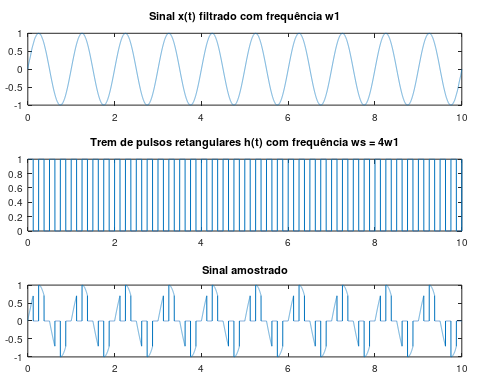
\includegraphics[width=4cm]{ex_amostrando.png} % leia abaixo
\caption{Obtenção do sinal amostrado $x$$_s$$(t)$ a partir de um sinal de pulsos retangulares $h(4w$$_1$$\cdot t)$.}
\end{figure}

\subsubsection{Replicação dos espectros}

Uma vez obtido o sinal amostrado$^{[8]}$ $x$$_s$$(t)$, deve-se novamente utilizar a FFT$^{[9]}$ para obter $X$$_s$$(\omega)$, e é neste ponto que ocorre o fenômeno da replicação dos espectros. Como a amostragem não é feita com impulsos ideais, as réplicas também não são ideias. Dessa forma, suas amplitudes são gradativamente atenuadas tendendo à zero.

\begin{figure}[H]
\captionsetup{justification=centering}
\centering % para centralizarmos a figura
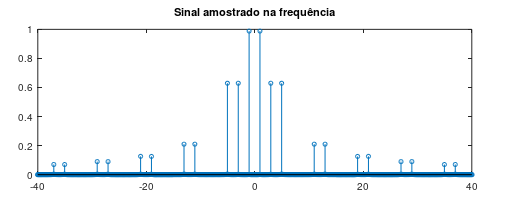
\includegraphics[width=4cm]{ex_replicacao.png} % leia abaixo
\caption{Sinal $x$$_s$$(t)$ na frequência. Com o gráfico ampliado, é possível perceber múltiplos pares de réplicas da frequência original, mas que são gradativamente atenuadas.}
\end{figure}

\subsection{Reconstrução do Sinal Amostrado}

\subsubsection{Filtro de reconstrução}

Através do sinal amostrado em frequência $X$$_s$$(\omega)$$^{[10]}$, o próximo passo, como o próprio diagrama ilustra, é aplicar um filtro de reconstrução$^{[11]}$ para obter a frequência original $w$$_1$ do sinal $x$$_f$$(t)$. Este processo não difere do já abordado filtro \textit{anti-aliasing}. Neste caso, o filtro ideal é aplicado no intervalo em que se encontra o espectro de frequência de interesse e tentando, o máximo possível, evitar réplicas parasitas.

\begin{figure}[H]
\captionsetup{justification=centering}
\centering % para centralizarmos a figura
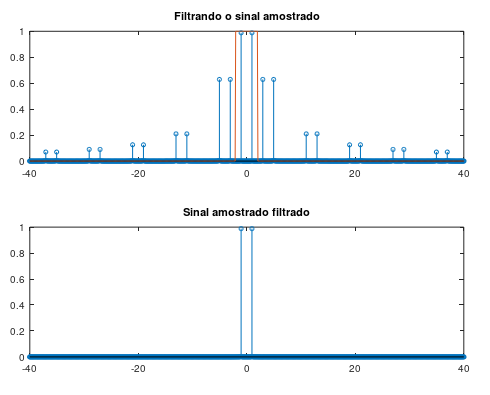
\includegraphics[width=4cm]{ex_filtrando_amostr.png} % leia abaixo
\caption{Filtro de recuperação (em laranja) aplicado em $X$$_s$$(\omega)$. No gráfico inferior, o sinal filtrado com o componente de frequência original $w$$_1$.}
\end{figure}

\subsubsection{Sinal recuperado}

Por fim, basta aplicar IFFT$^{[12]}$ em $X$$_s$$(\omega)$ filtrado para reconstruir o sinal $x$$_f$$(t)$. O resultado desta operação é a saída do sistema$^{[13]}$, que equivale a senóide $x$$_1$.

\begin{figure}[H]
\captionsetup{justification=centering}
\centering % para centralizarmos a figura
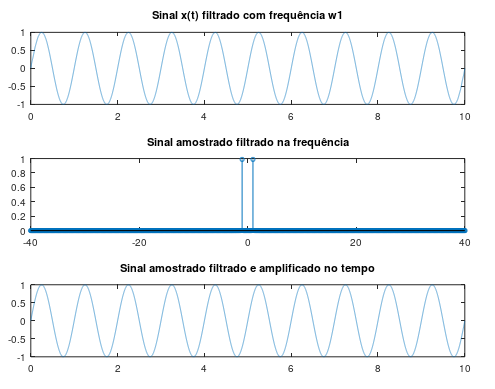
\includegraphics[width=4cm]{ex_amplificando_amostr.png} % leia abaixo
\caption{Comparação entre $x$$_f$$(t)$ com o sinal amostrado $x$$_s$$(t)$ após a filtragem e amplificação.}
\end{figure}

\section{Resultados e Discussões}

\subsection{Aliasing}

Vamos tomar como exemplo um sinal $x(t)$ formado pela soma de três senoides com frequências $w_1 = 10 Hz$, $w_2 = 50 Hz$ e $w_3 = 90 Hz$.

\begin{figure}[H]
\captionsetup{justification=centering}
\centering % para centralizarmos a figura
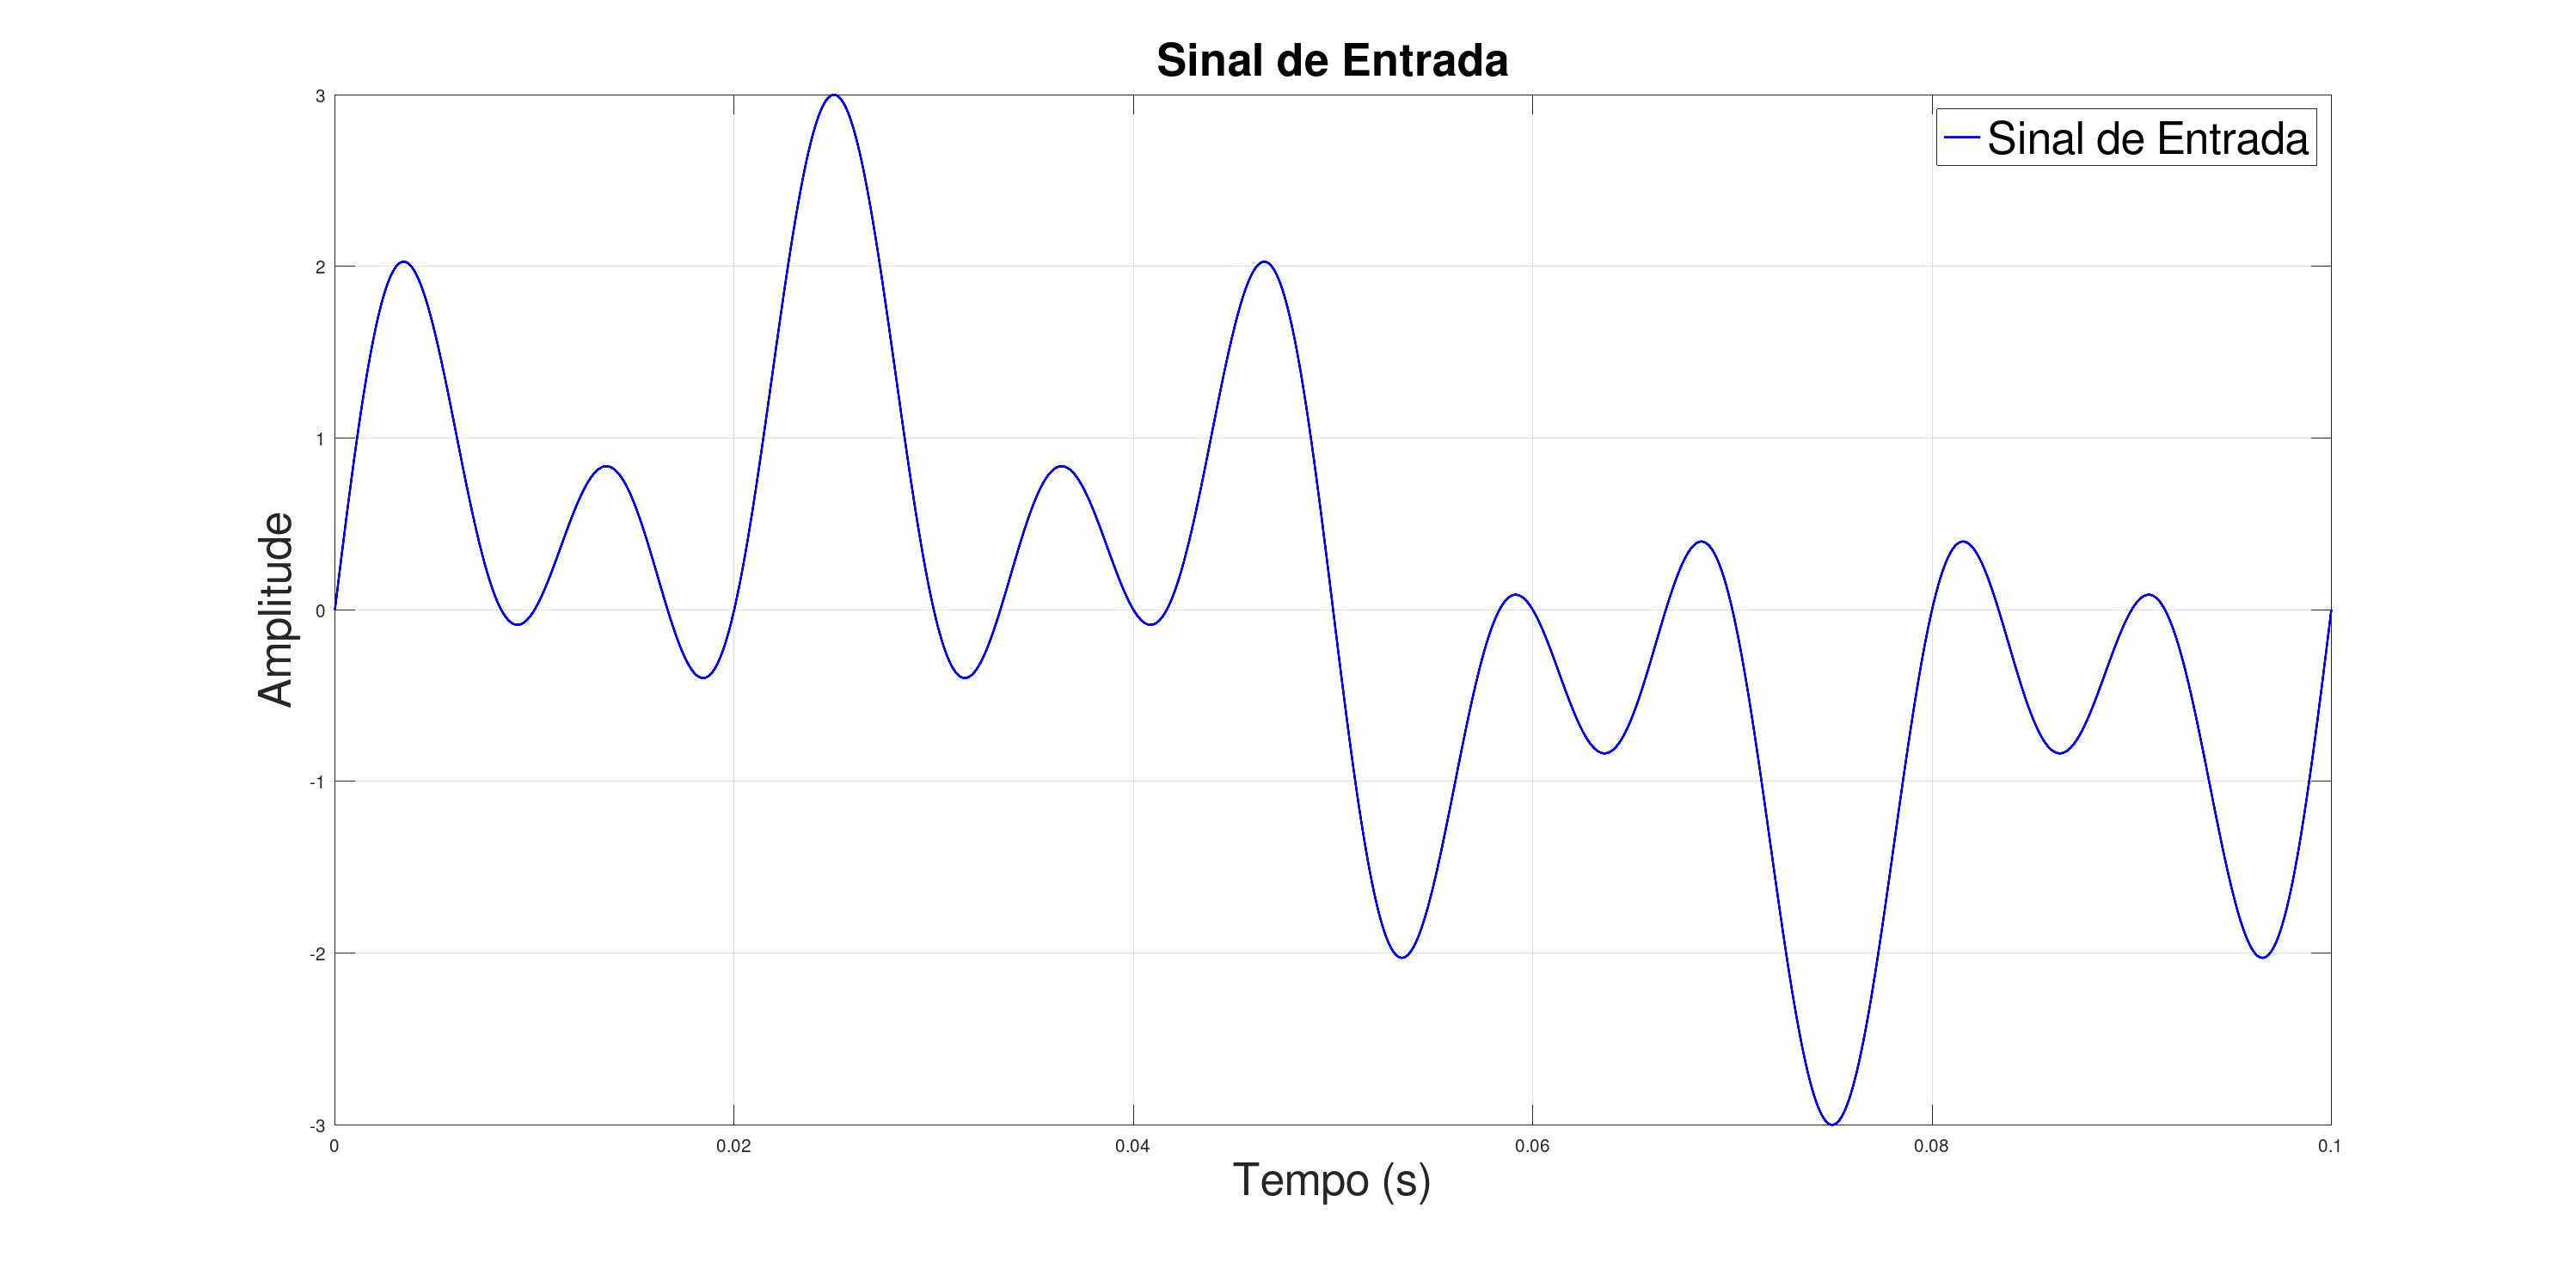
\includegraphics[width=7cm]{sinal_entrada_00.jpg} % leia abaixo
\caption{Sinal de entrada $x(t)$ formado pela soma de três senoides.}
\end{figure}

O sinal resultado possui período igual ao menor período dos sinais somados. Neste caso, $P_{min} = 0.1s$. Portanto, o sinal resultante possui período $P = 0.1s$. Apesar da entrada ter esta característica, o sinal no qual queremos trabalhar possui frequência $f = 10Hz$. Então todo e qualquer sinal fora desta frequência é considerado ruído. Para continuar é preciso remover esses ruídos para que eles não atrapalhem o nosso processamento. Vamos utilizar um filtro passa-baixas ideal com frequência de corte $w_c = 15Hz$, ele irá remover as frequências indesejadas, deixando apenas a frequência a ser utilizada.

\begin{figure}[H]
\captionsetup{justification=centering}
\centering % para centralizarmos a figura
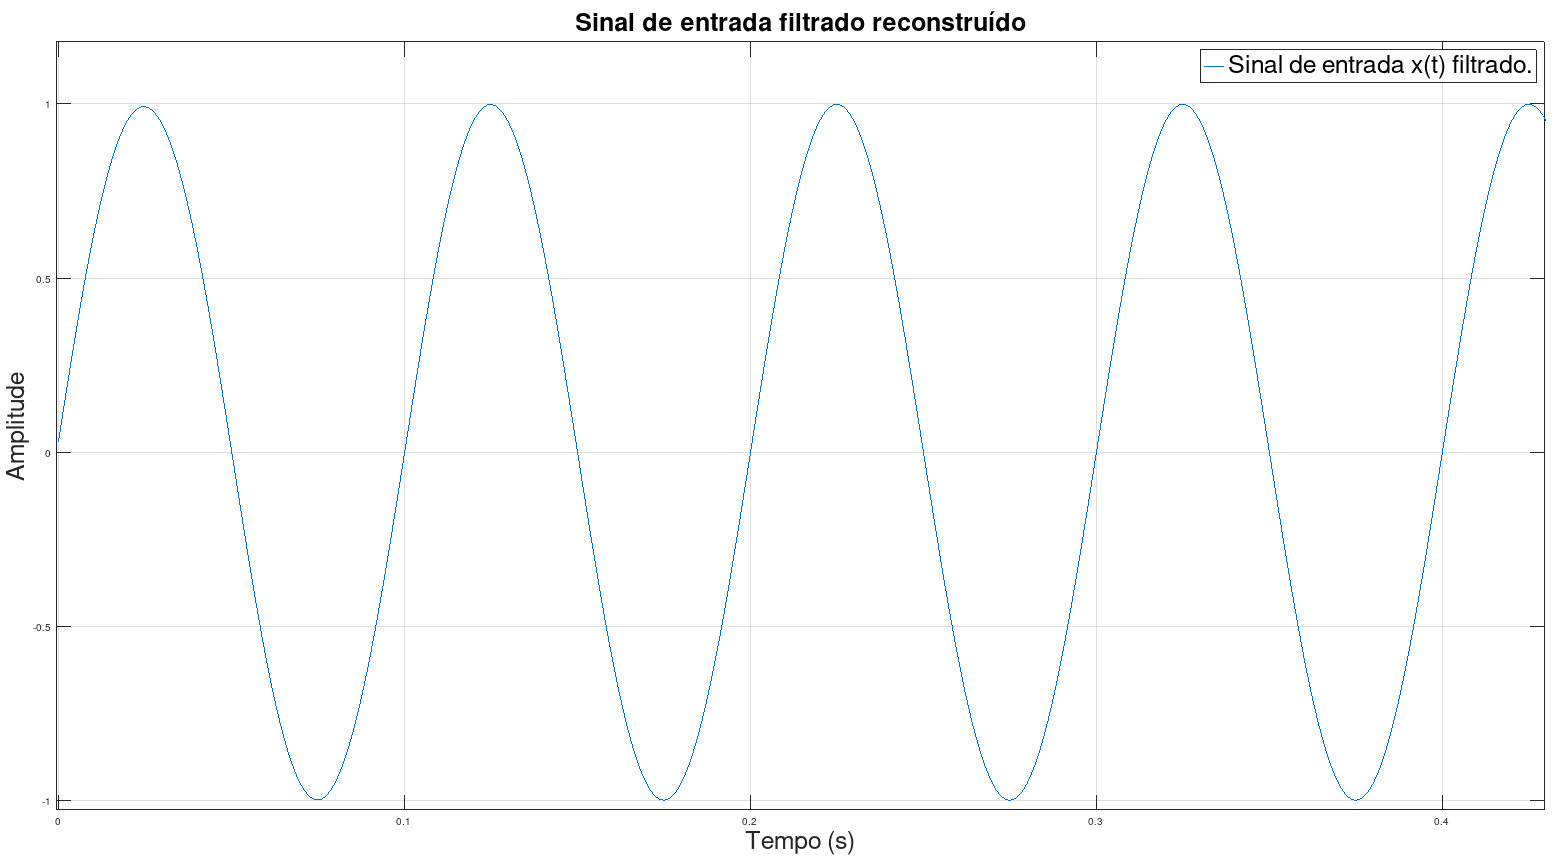
\includegraphics[width=6cm]{sinal_entrada_10Hz.png} % leia abaixo
\caption{Sinal de entrada $x(t)$ filtrado.}
\end{figure}

Agora que foi removido todo ruído, podemos amostrar o sinal. Sabendo que o teorema de \textit{Nyquist} determina a frequência de amostragem ideal, ou seja, temos que ter uma amostragem $w_{m} > 2\cdot w_{s}$.

\subsection{Amostragem e Reconstrução}

Vamos utilizar um trem de pulsos retangulares com frequência $w_s = 40Hz$. Como a frequência de amostragem é maior que o dobro da frequência do sinal, não haverá \textit{aliasing}. O sinal amostrado é dado por $x_s(t) = x(t) \cdot h(t)$, onde $h(t)$ é o trem de pulsos retangulares. O sinal amostrado é o seguinte:

\begin{figure}[H]
\captionsetup{justification=centering}
\centering % para centralizarmos a figura
\includegraphics[width=6cm]{sinal_amostrado_40hz.png} % leia abaixo
\caption{Sinal amostrado $x_s(t)$.}
\end{figure}

Olhando o espectro deste sinal podemos observar a replicação causado pela amostragem:

\begin{figure}[H]
\captionsetup{justification=centering}
\centering % para centralizarmos a figura
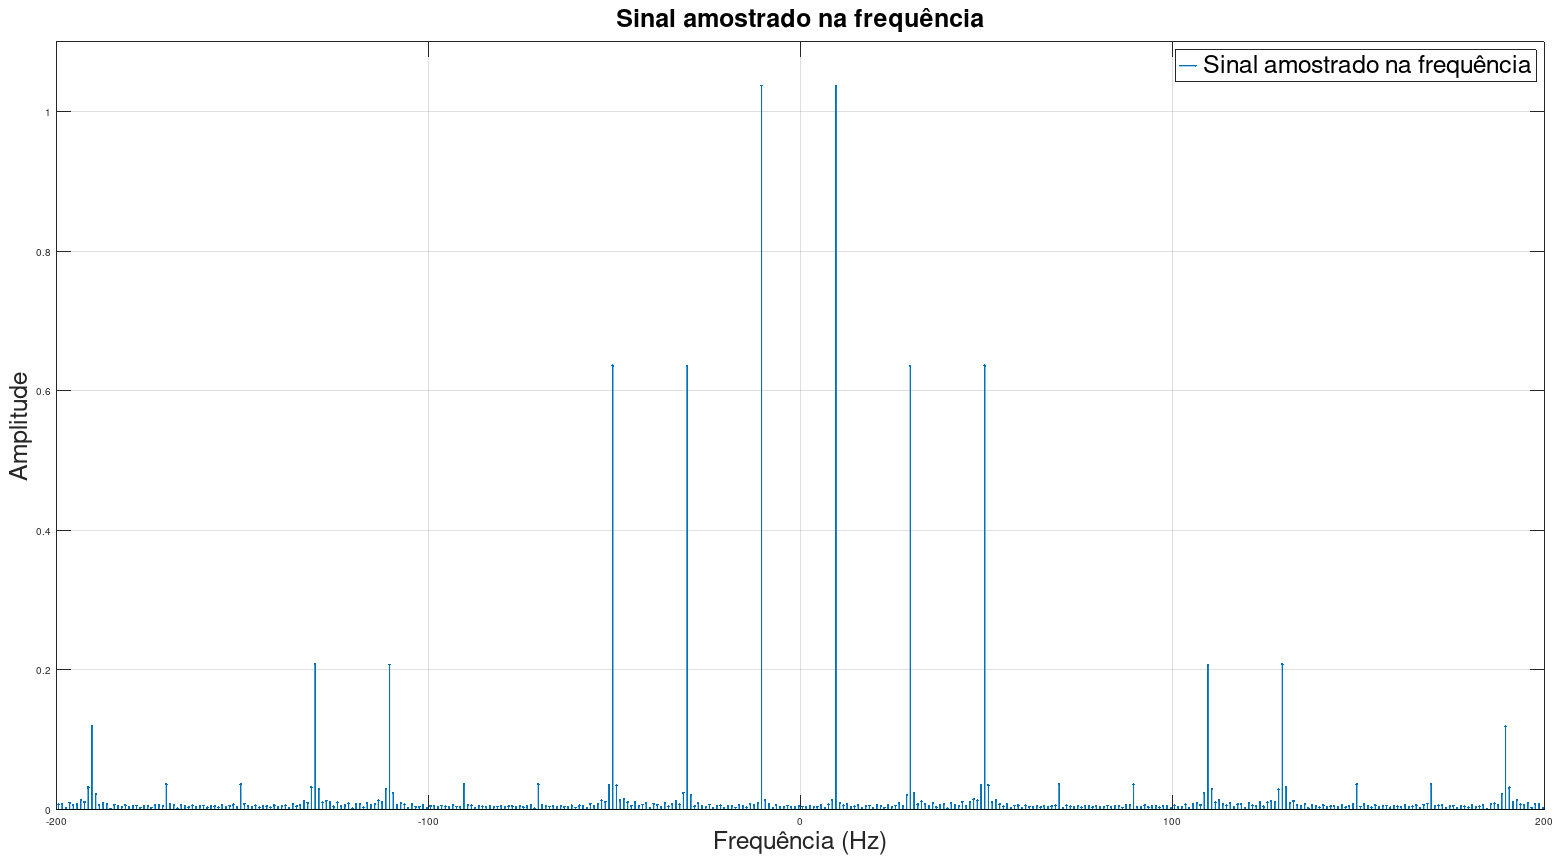
\includegraphics[width=6cm]{sinal_amostrado_frequencia_40Hz.png} % leia abaixo
\caption{Frequência do sinal amostrado $F_s(t)$.}
\end{figure}

Para remover essas frequências, vamos utilizar um filtro passa-baixas ideal com frequência de corte $w_c = 15Hz$. O sinal filtrado é dado por $x_f(t) = x_s(t) \cdot h_s(t)$, onde $h_s(t)$ é o filtro passa-baixas ideal(fig. \ref*{fig:filtro_reconstrucao}). O sinal filtrado é o seguinte:

\begin{figure}[H]
\captionsetup{justification=centering}
\centering % para centralizarmos a figura
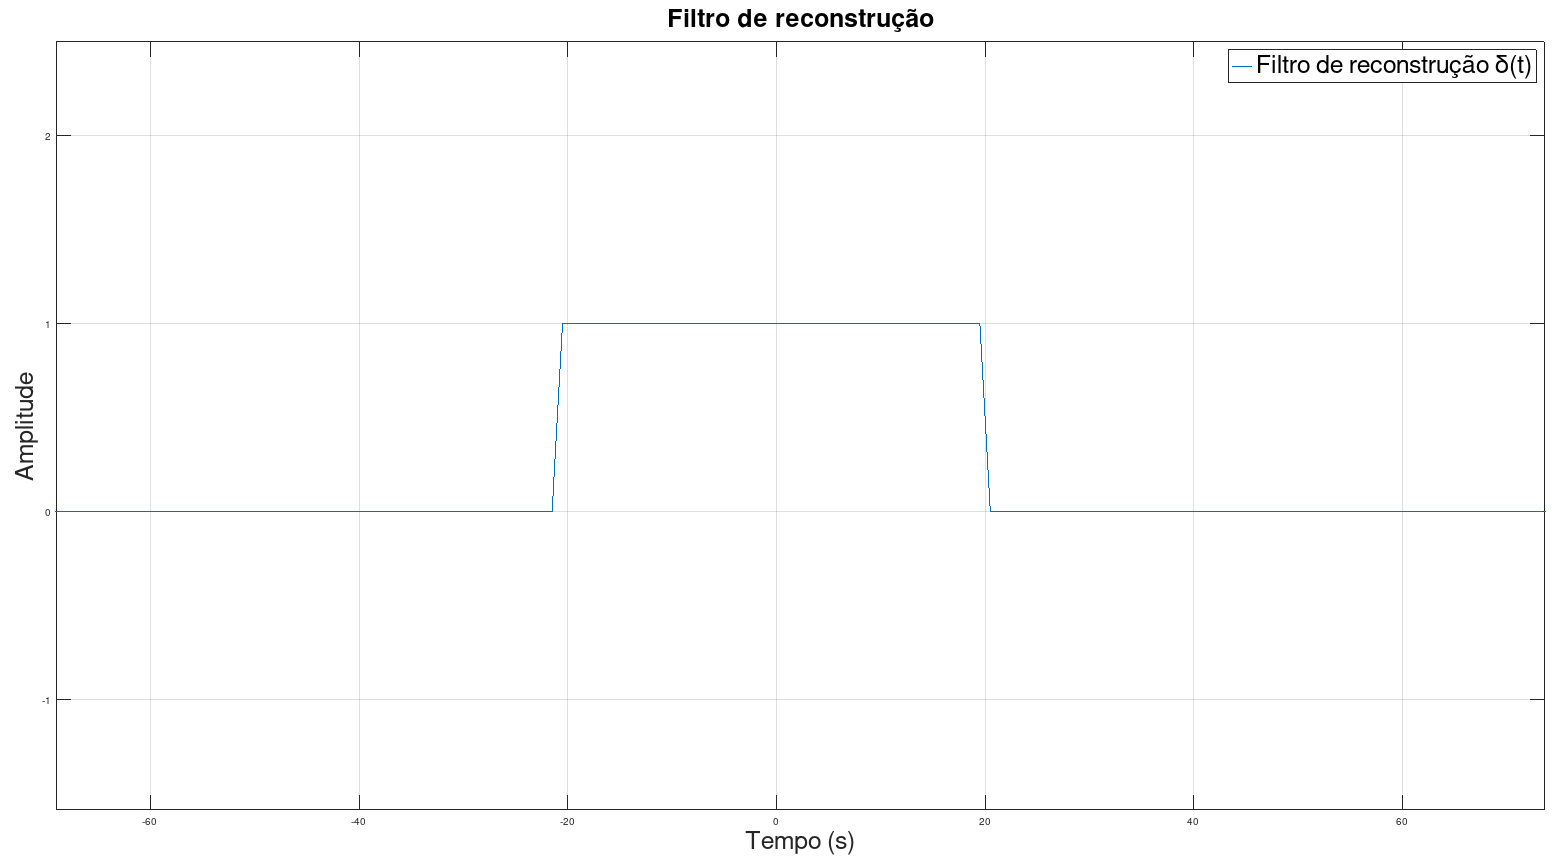
\includegraphics[width=6cm]{filtro_reconstrucao.png} % leia abaixo
\caption{Filtro de reconstrução $h_s(t)$.}
\label{fig:filtro_reconstrucao}
\end{figure}

\begin{figure}[H]
\captionsetup{justification=centering}
\centering % para centralizarmos a figura
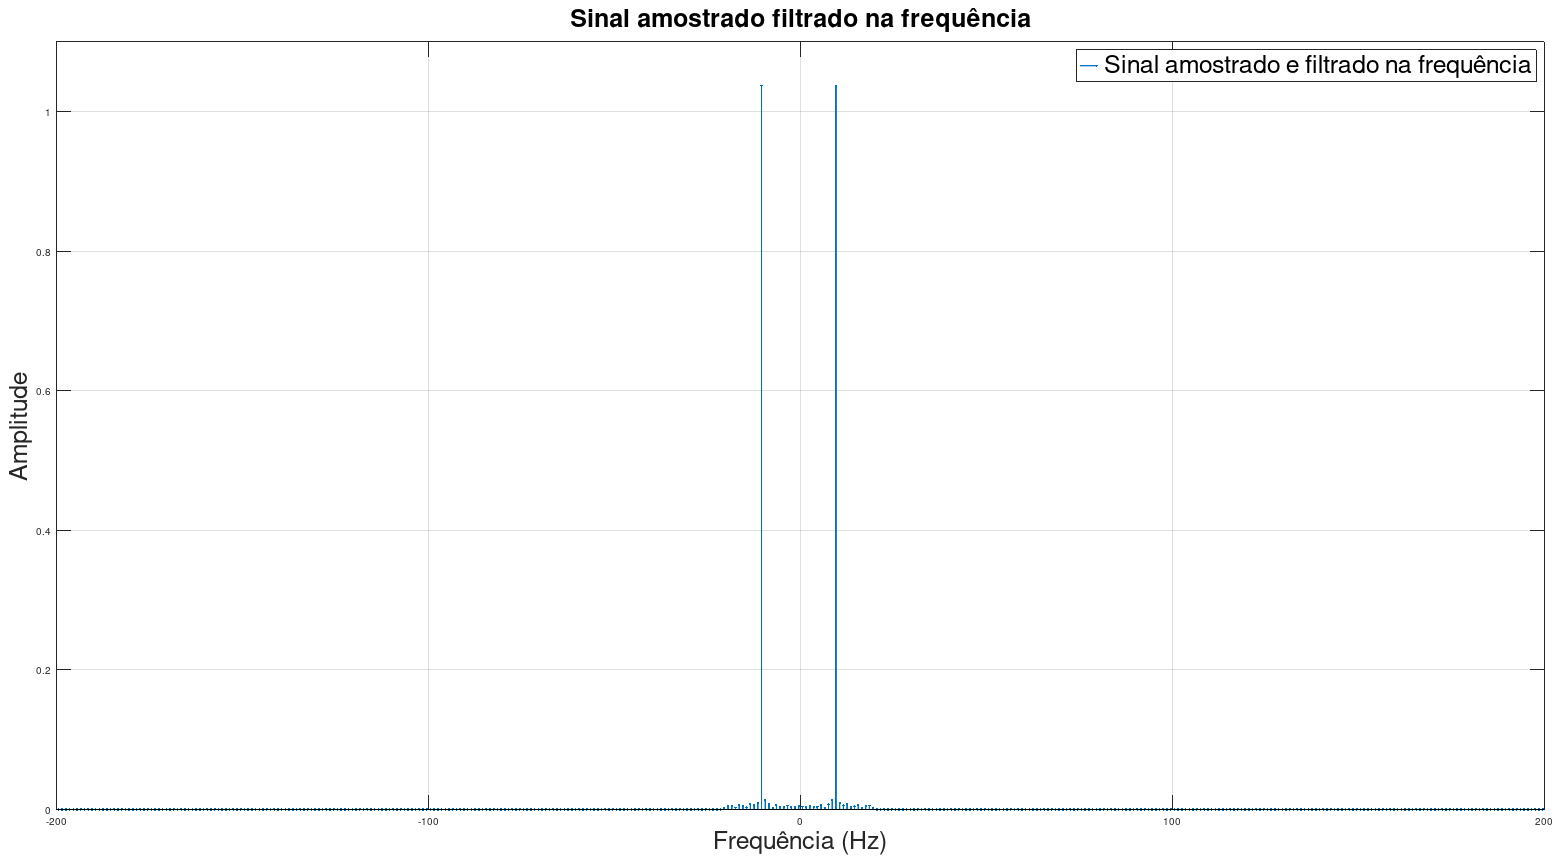
\includegraphics[width=6cm]{sinal_amostrado_filtrado_frequencia_40Hz.png} % leia abaixo
\caption{Frequência do sinal amostrado filtrado pelo filtro de reconstrução $h_s(t)$.}
\end{figure}

Removendo as frequências indesejadas, podemos reconstruir o sinal original. Para isso, vamos utilizar a transformada rápida inversa de fourier. O sinal reconstruído é dado por $x_r(t) = ifft(X_f(\omega))$, onde $X_f(\omega)$ é a transformada rápida de fourier do sinal filtrado. O sinal reconstruído é o seguinte:

\begin{figure}[H]
\captionsetup{justification=centering}
\centering % para centralizarmos a figura
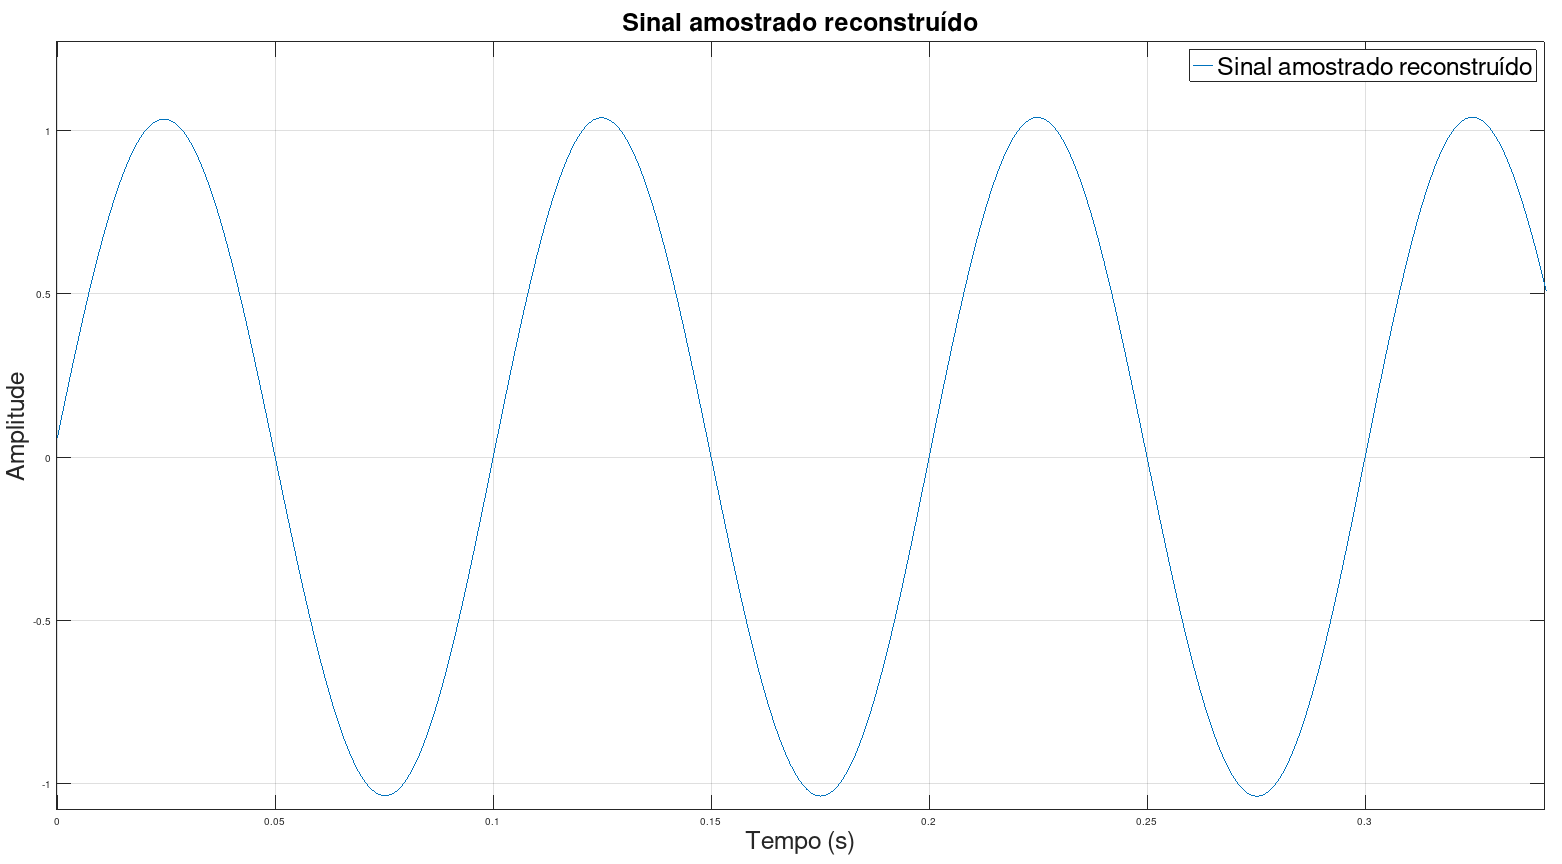
\includegraphics[width=6cm]{sinal_reconstruido_40Hz.png} % leia abaixo
\caption{Sinal reconstruído $x_r(t)$.}
\end{figure}

Para observar na prática a amostragem do sinal com uma frequência inferior a frequência de Nyquist, vamos utilizar um trem de pulsos retangulares com frequência $w_s = 5Hz$. Como a frequência de amostragem é menor que o dobro da frequência do sinal, haverá \textit{aliasing}. Vamos manter todos os outros parâmetros iguais ao exemplo anterior. Para observar apenas o efeito do \textit{aliasing}. Utilizando o trem de pulsos, o sinal amostrado é o seguinte:

\begin{figure}[H]
\captionsetup{justification=centering}
\centering % para centralizarmos a figura
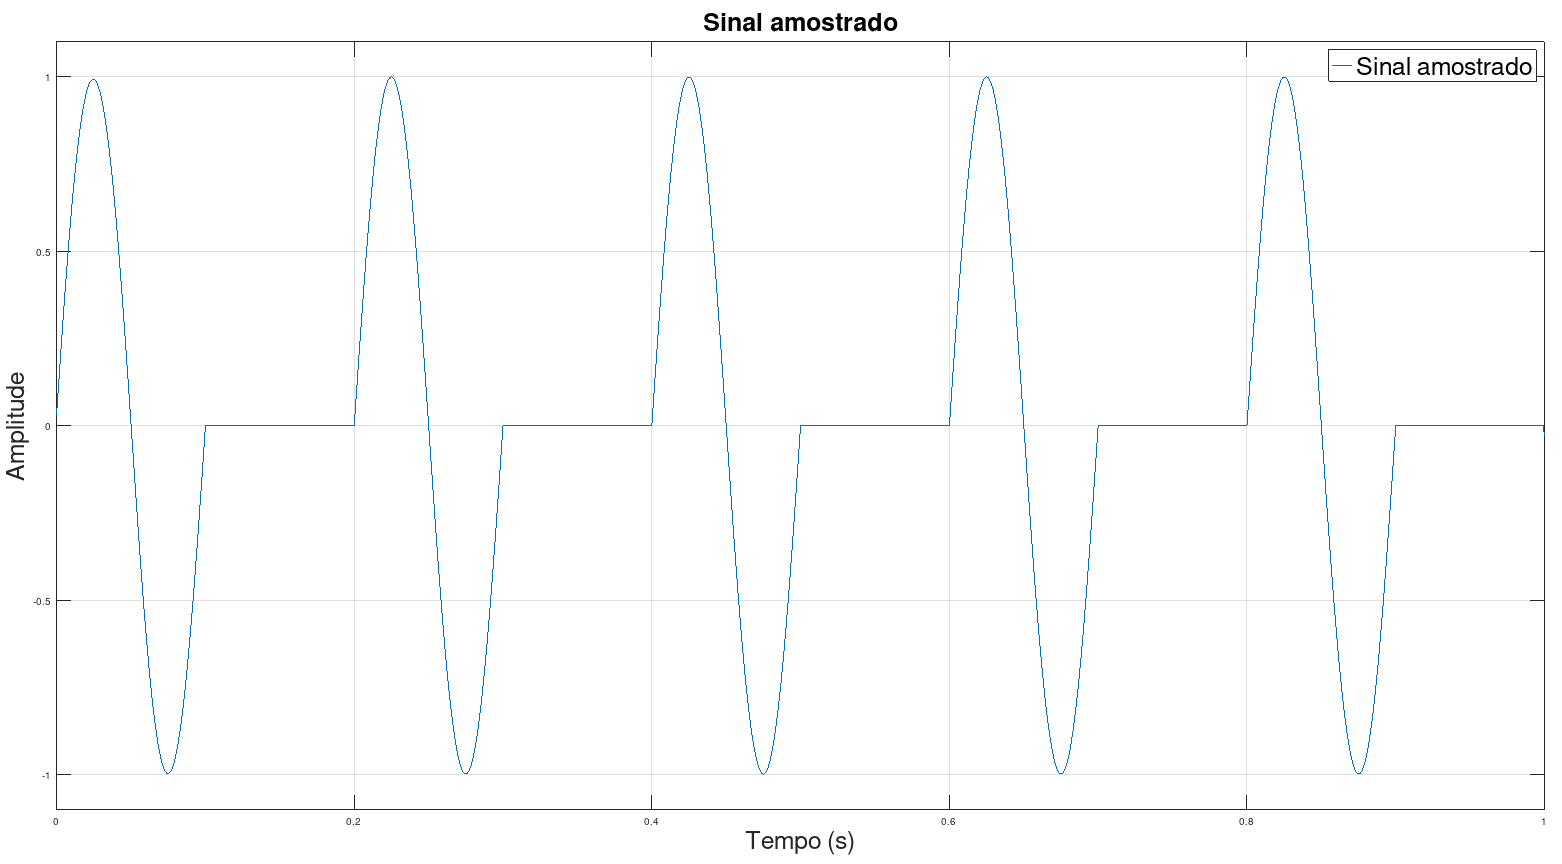
\includegraphics[width=6cm]{sinal_amostrado_5Hz.png} % leia abaixo
\label{fig:sinal_amostrado_5Hz}
\caption{Sinal amostrado $5Hz$.}
\end{figure}

O legal de utilizar a frequência de amostragem a metade do sinal de entrada é poder observar o efeito do \textit{aliasing}, na figura \ref{fig:sinal_amostrado_5Hz}, vemos que metade do sinal é perdido. Olhando o espectro deste sinal podemos observar a replicação causado pela amostragem, o cenário seria ainda pior se o sinal original tivesse mais frequências, eles também seriam replicados. E observando na frequência, mesmo que apliquemos o filtro de reconstrução, não vamos conseguir remover os espectros indesejados, pois eles estão sobrepostos.

\begin{figure}[H]
\captionsetup{justification=centering}
\centering % para centralizarmos a figura
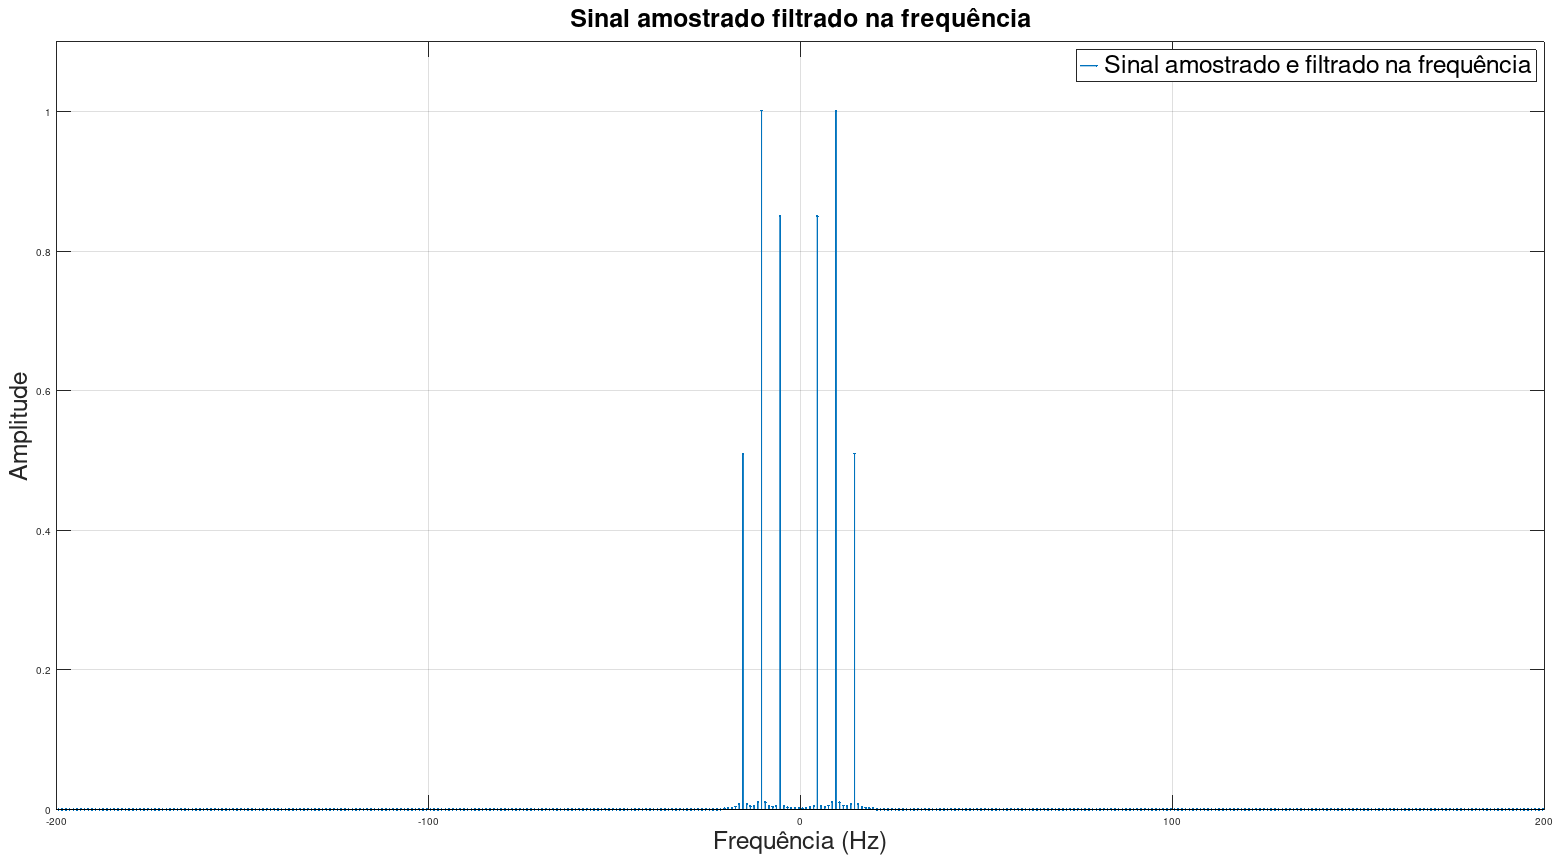
\includegraphics[width=6cm]{sinal_amostrado_filtrado_frequencia_5Hz.png} % leia abaixo
\caption{Sinal amostrado filtrado na frequência $5Hz$.}
\end{figure}

Reconstruindo o sinal, podemos observar que o sinal reconstruído não é igual ao sinal original, pois o sinal original foi perdido durante a amostragem. Observando o sinal reconstruído, notamos que é um sinal completamente diferente do sinal de entrada.

\begin{figure}[H]
\captionsetup{justification=centering}
\centering % para centralizarmos a figura
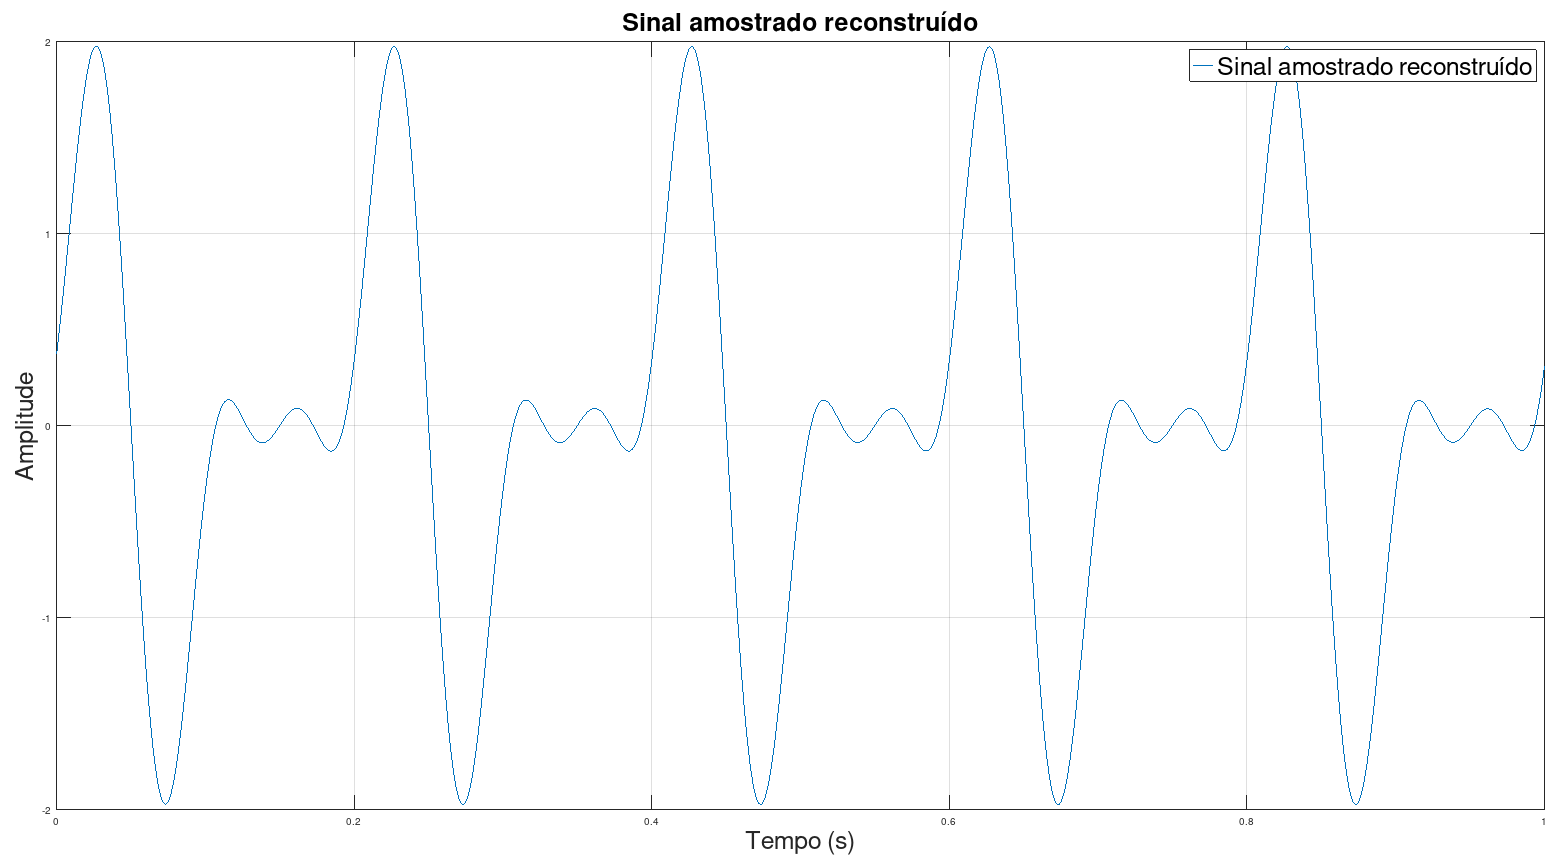
\includegraphics[width=6cm]{sinal_reconstruido_5Hz.png} % leia abaixo
\caption{Sinal amostrado reconstruído $5Hz$.}
\end{figure}

Agora comparando lado a lado, o sinal reconstruído e o sinal original de entrada na figura \ref{fig:comparacao_5H_sinal_original} em azul e vermelho, respectivamente, observamos o efeito da amostragem na amplitude, causado pela sobreposição dos espectros.

\begin{figure}[H]
\captionsetup{justification=centering}
\centering % para centralizarmos a figura
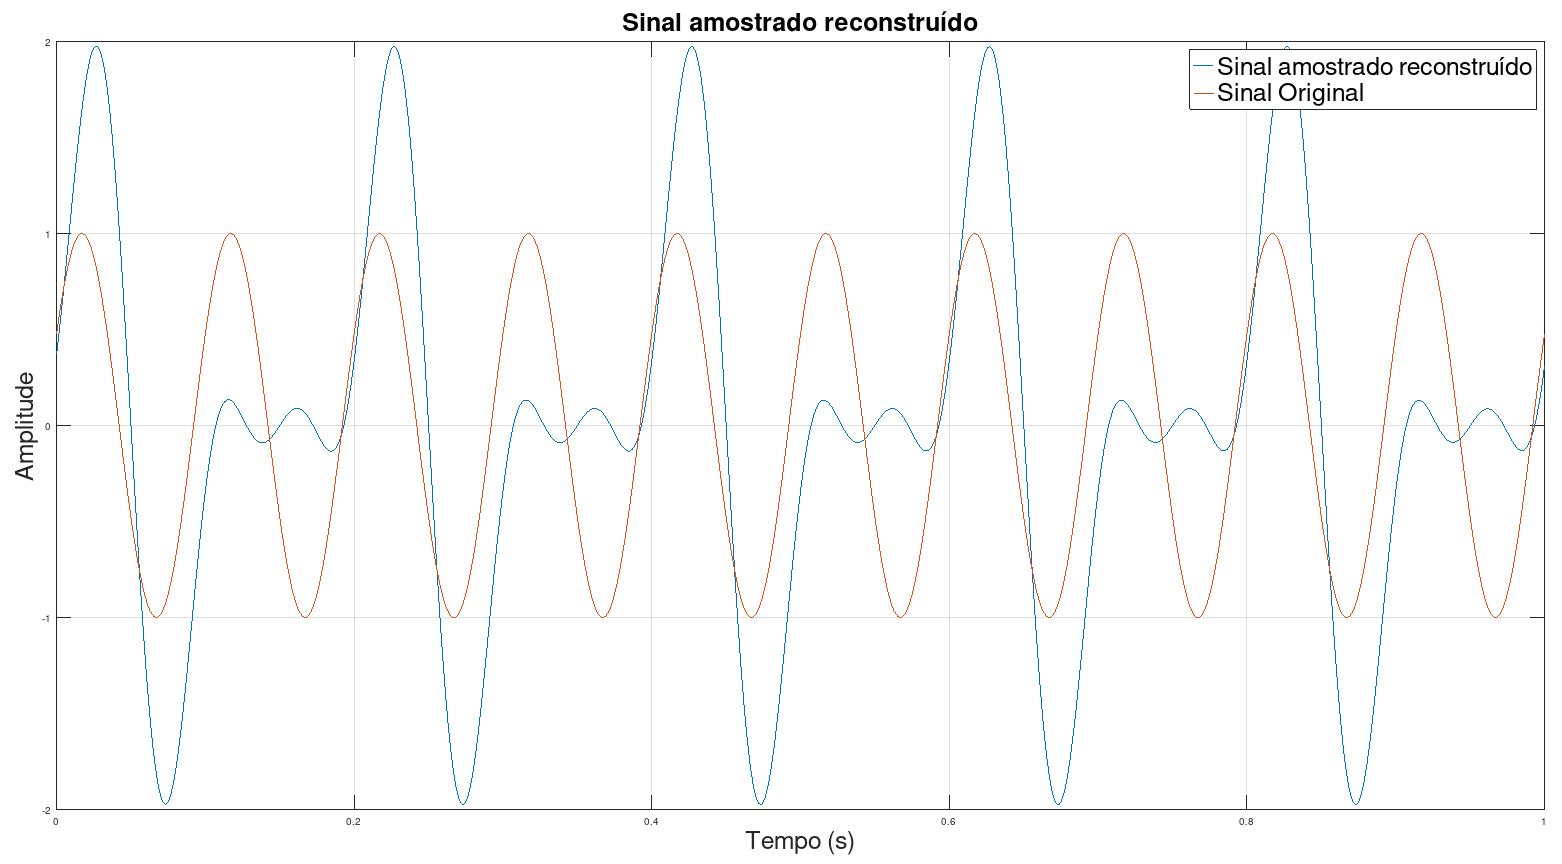
\includegraphics[width=6cm]{comparacao_5H_sinal_original.png} % leia abaixo
\label{fig:comparacao_5H_sinal_original}
\caption{Comparação do sinal reconstruído $5Hz$ e o sinal de entrada $10Hz$.}
\end{figure}

Utilizar esse sinal para o transporte de informações não seria uma opção, pois todo sinal é corrompido e o processamento digital deste sinal não iria obter sucesso.

\section{Conclusão}

% references section

% can use a bibliography generated by BibTeX as a .bbl file
% BibTeX documentation can be easily obtained at:
% http://mirror.ctan.org/biblio/bibtex/contrib/doc/
% The IEEEtran BibTeX style support page is at:
% http://www.michaelshell.org/tex/ieeetran/bibtex/
%\bibliographystyle{IEEEtran}
% argument is your BibTeX string definitions and bibliography database(s)
%\bibliography{IEEEabrv,../bib/paper}
%
% <OR> manually copy in the resultant .bbl file
% set second argument of \begin to the number of references
% (used to reserve space for the reference number labels box)
\bibliographystyle{IEEEtran}
\bibliography{bibtex/bib/IEEEabrv,bibtex/bib/IEEEexample}

\end{document}


